% Created 2013-01-17 Thu 19:29
\documentclass[bigger]{beamer}
\usepackage[utf8]{inputenc}
\usepackage[T1]{fontenc}
\usepackage{fixltx2e}
\usepackage{graphicx}
\usepackage{longtable}
\usepackage{float}
\usepackage{wrapfig}
\usepackage{soul}
\usepackage{textcomp}
\usepackage{marvosym}
\usepackage{wasysym}
\usepackage{latexsym}
\usepackage{amssymb}
\usepackage{hyperref}
\tolerance=1000
\titlegraphic{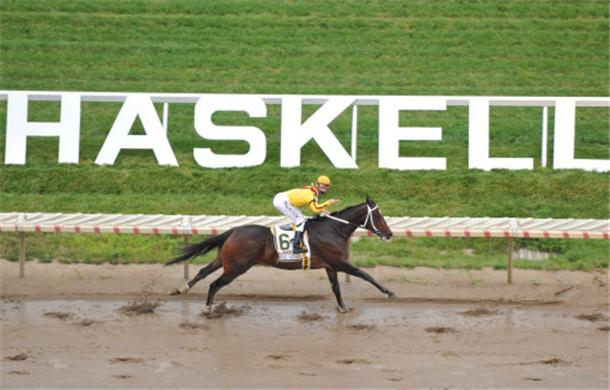
\includegraphics{../pictures/haskell_horse.jpg}}
\setbeamertemplate{navigation symbols}{}
\mode<beamer>{\usetheme{CambridgeUS}}
\institute[GWU]{The George Washington University}
\usepackage{listings}
\lstset{language=Haskell, basicstyle=\scriptsize}
\providecommand{\alert}[1]{\textbf{#1}}

\title{70\% Demonstration}
\author{Andrew Hirsch}
\date{Thursday, January 17, 2013 }
\hypersetup{
  pdfkeywords={},
  pdfsubject={},
  pdfcreator={Emacs Org-mode version 7.8.11}}

\begin{document}

\maketitle



\begin{frame}
\frametitle{The Life of a spy}
\label{sec-1}

\begin{itemize}
\item Imagine a spy, Alice
\item She has to pass messages on to her fellow, Bob
\item But they can only be so long!
\item She can tell the spy where to go for a (longer) message
\item She packages up the longer messages and tells Bob where to go
\end{itemize}
\end{frame}
\begin{frame}
\frametitle{The troubles of space}
\label{sec-2}

\begin{itemize}
\item But, now, Alice has a limited area she is permitted to move in (her handlers keep her on a tight leash)
\item She only have a bit of overlap with Bob
\item She has to give them directions to get to a longer message in the shared area
\end{itemize}
\end{frame}
\begin{frame}
\frametitle{The Problem with Composite Functions}
\label{sec-3}

\begin{itemize}
\item This is exactly what happens in the Composite operating system
\item Composite is made up of ``components'', which only have a limited shared space
\item They can only talk to each other in such long messages
\end{itemize}
\end{frame}
\begin{frame}
\frametitle{Coding the Solution}
\label{sec-4}

\begin{itemize}
\item The solution is worse than the problem
\item There is a lot of sticky code that has to be perfectly hand-written!
\item This is where we automate
\end{itemize}
\end{frame}
\begin{frame}
\frametitle{Automating stub generation}
\label{sec-5}

\begin{itemize}
\item Pony is good at this sort of automation
\item Anywhere there's a function that should be called between components, automatically generate \emph{stubs}
\item These stubs tell how to package and address messages in shared memory
\end{itemize}
\end{frame}
\begin{frame}
\frametitle{Is there a need for extra syntax?}
\label{sec-6}

\begin{itemize}
\item It is common to add extra syntax here
\item This is called an \emph{Interface Description Language}
\item If we need extra syntax, we will have to add it in to Pony by hand
\end{itemize}
\end{frame}
\begin{frame}
\frametitle{Protocols}
\label{sec-7}

\begin{itemize}
\item Let us return to Alice and Bob
\item How are they to speak to each other?
\item They use a well defined \emph{protocol} that they can each react to
\item Then they always know what the other is saying
\end{itemize}
\end{frame}
\begin{frame}
\frametitle{Composing Machines}
\label{sec-8}

\begin{itemize}
\item Imagine that there is a machine that given a red widget should always return a blue one
\item And a second machine that given a blue widget, should always return a green one
\item We can make a green widget from a red one by giving the red widget to the first machine
\item Then putting the resulting blue widget in the second!
\end{itemize}
\end{frame}
\begin{frame}
\frametitle{Contracts}
\label{sec-9}

\begin{itemize}
\item The kind of promises given by the first machine are known as contracts
\item They can be enforced by a programming language when given by a function
\item This is important when promises \underline{must} be kept, such as in an OS
\end{itemize}
\end{frame}
\begin{frame}
\frametitle{Protocols in Composite}
\label{sec-10}

\begin{itemize}
\item Composite components should use protocols
\item That way they talk to each other in sane ways
\item But, they should know how they respond to different inputs
\item This should be enforced by contracts
\end{itemize}
\end{frame}
\begin{frame}
\frametitle{Contract Language}
\label{sec-11}

\begin{itemize}
\item Functions that are called by other components should implement protocols
\item It needs to be enforced that sticks to a protocol
\item A protocol language that it is easy to enforce speaking in
\end{itemize}
\end{frame}
\begin{frame}
\frametitle{The Plan Going Forward}
\label{sec-12}

\begin{itemize}
\item Create transformation for stub generation
\item Design extra syntax (with Composite team)
\item Create fork of pony parser to deal with extra syntax
\item Create transformations for extra syntax
\item Design protocol language (with Composite team)
\item Create fork of pony parser to deal with protocol language
\item Create transformation for protocol language
\end{itemize}
\end{frame}

\end{document}
